% Drawing 144/03-8 -- folder 144, batch 03, archive page 59 (PDF page 60).
% Transcription: Une figure de dix triangles autour d'un triangle central $r$ (sommets étiquetés $0$, $1$, $\infty$ de manière à alterner), chacun marqué du repère qu'il représente et de son sens de rotation : $\tau_{0}r$, $\tau_{1}r$, $\tau_{\infty}r$, $\tau_{1}\tau_{\infty}r = \rho_{0}^{-1}r$, $\tau_{\infty}\tau_{1}r = \rho_{0}r$, $\tau_{0}\tau_{1}r = \rho_{\infty}^{-1}r$, $\tau_{1}\tau_{0}r = \rho_{\infty}r$, $\tau_{0}\tau_{\infty}r = \rho_{1}r$, $\tau_{\infty}\tau_{0}r = \rho_{1}^{-1}r$ ; les arêtes portent des flèches d'orientation.
% Kind: ten triangles of frames around r (piece of a triangulation). Method 3 (encoded, rendered from the data). Status: partial.
% Notes: Encoded as polyhedron/1 (a disc: 12 vertices, 21 edges, 10 triangles, chi = 1); every triangle has one vertex of each type 0, 1, infinity. Rendered with the vertices placed once and every edge drawn between them. Each edge carries one arrowhead, as on the page; read on the facsimile, all 21 go 0 -> 1 -> infinity -> 0, and they are drawn from that rule. Labels \small, placed where he wrote them: the vertex types (the far left vertex carries no label on the page; its type 0 is the alternation) and the frames r, tau_0 r, tau_1 r, tau_infty r, tau_1 tau_infty r = rho_0^{-1} r, tau_infty tau_1 r = rho_0 r, tau_0 tau_infty r = rho_1 r, tau_0 tau_1 r = rho_infty^{-1} r, tau_infty tau_0 r = rho_1^{-1} r, tau_1 tau_0 r = rho_infty r. Still differs from the facsimile: the small rotation arrow of each frame is not drawn (their senses are not legible with certainty). The stroke "5" above at the right is not part of the figure. Redrawn 2026-11-09 (issue 128): to check again.
% Coordinates: 1 unit = 1 mm = 1/100 of the crop width (bbox in page fractions: [0.25, 0.06, 0.57, 0.32]).
% Redrawn by Claude (claude-opus-5-5), issue #73, 2026-11-09; not checked by a human; not compiled (no TeX in the session).
% Rights: reproduces part of the work -- behind RENDER_TRANSCRIPTS, never published by itself.
\documentclass[tikz,border=3pt]{standalone}
\usepackage{amsmath,amssymb}
\usetikzlibrary{patterns,arrows.meta}
\tikzset{pencil/.style={black!45}, struck/.style={black!35}, mark/.style={circle,draw,inner sep=1.3pt}, pt/.style={circle,fill,inner sep=0.9pt}, opt/.style={circle,draw,fill=white,inner sep=1.1pt}}
\begin{document}
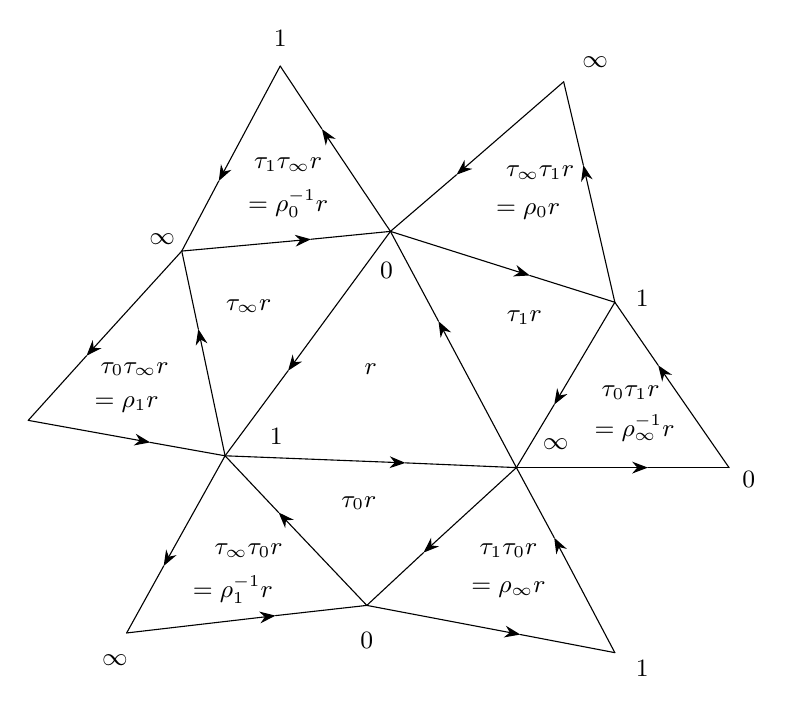
\begin{tikzpicture}[x=1mm,y=1mm,line cap=round,line join=round,font=\scriptsize]
\draw[-{Stealth[length=2mm]}] (48,-49) -- (35,-66.7);
\draw (35,-66.7) -- (27,-77.5);
\draw[-{Stealth[length=2mm]}] (64,-79) -- (54.1,-60.4);
\draw (54.1,-60.4) -- (48,-49);
\draw[-{Stealth[length=2mm]}] (48,-49) -- (39.3,-36);
\draw (39.3,-36) -- (34,-28);
\draw[-{Stealth[length=2mm]}] (21.5,-51.5) -- (37.9,-50);
\draw (37.9,-50) -- (48,-49);
\draw[-{Stealth[length=2mm]}] (70,-30) -- (56.4,-41.8);
\draw (56.4,-41.8) -- (48,-49);
\draw[-{Stealth[length=2mm]}] (48,-49) -- (65.7,-54.6);
\draw (65.7,-54.6) -- (76.5,-58);
\draw[-{Stealth[length=2mm]}] (27,-77.5) -- (49.9,-78.4);
\draw (49.9,-78.4) -- (64,-79);
\draw[-{Stealth[length=2mm]}] (27,-77.5) -- (23.6,-61.4);
\draw (23.6,-61.4) -- (21.5,-51.5);
\draw[-{Stealth[length=2mm]}] (2,-73) -- (17.5,-75.8);
\draw (17.5,-75.8) -- (27,-77.5);
\draw[-{Stealth[length=2mm]}] (27,-77.5) -- (19.2,-91.5);
\draw (19.2,-91.5) -- (14.5,-100);
\draw[-{Stealth[length=2mm]}] (45,-96.5) -- (33.8,-84.7);
\draw (33.8,-84.7) -- (27,-77.5);
\draw[-{Stealth[length=2mm]}] (76.5,-58) -- (68.8,-71);
\draw (68.8,-71) -- (64,-79);
\draw[-{Stealth[length=2mm]}] (64,-79) -- (52.2,-89.8);
\draw (52.2,-89.8) -- (45,-96.5);
\draw[-{Stealth[length=2mm]}] (76.5,-102.5) -- (68.8,-87.9);
\draw (68.8,-87.9) -- (64,-79);
\draw[-{Stealth[length=2mm]}] (64,-79) -- (80.7,-79);
\draw (80.7,-79) -- (91,-79);
\draw[-{Stealth[length=2mm]}] (34,-28) -- (26.2,-42.6);
\draw (26.2,-42.6) -- (21.5,-51.5);
\draw[-{Stealth[length=2mm]}] (21.5,-51.5) -- (9.4,-64.8);
\draw (9.4,-64.8) -- (2,-73);
\draw[-{Stealth[length=2mm]}] (76.5,-58) -- (72.5,-40.6);
\draw (72.5,-40.6) -- (70,-30);
\draw[-{Stealth[length=2mm]}] (91,-79) -- (82,-66);
\draw (82,-66) -- (76.5,-58);
\draw[-{Stealth[length=2mm]}] (14.5,-100) -- (33.4,-97.8);
\draw (33.4,-97.8) -- (45,-96.5);
\draw[-{Stealth[length=2mm]}] (45,-96.5) -- (64.5,-100.2);
\draw (64.5,-100.2) -- (76.5,-102.5);
\node[inner sep=1pt] at (34,-24.5) {\small $1$};
\node[inner sep=1pt] at (74,-27.5) {\small $\infty$};
\node[inner sep=1pt] at (19,-50) {\small $\infty$};
\node[inner sep=1pt] at (47.5,-54) {\small $0$};
\node[inner sep=1pt] at (80,-57.5) {\small $1$};
\node[inner sep=1pt] at (33.5,-75) {\small $1$};
\node[inner sep=1pt] at (69,-76) {\small $\infty$};
\node[inner sep=1pt] at (93.5,-80.5) {\small $0$};
\node[inner sep=1pt] at (13,-103.5) {\small $\infty$};
\node[inner sep=1pt] at (45,-101) {\small $0$};
\node[inner sep=1pt] at (80,-104.5) {\small $1$};
\node[inner sep=1pt] at (35,-40.5) {\small $\tau_1\tau_\infty r$};
\node[inner sep=1pt] at (35,-45.5) {\small $=\rho_0^{-1}r$};
\node[inner sep=1pt] at (67,-41.5) {\small $\tau_\infty\tau_1r$};
\node[inner sep=1pt] at (65.5,-46.5) {\small $=\rho_0r$};
\node[inner sep=1pt] at (30,-58.5) {\small $\tau_\infty r$};
\node[inner sep=1pt] at (45.5,-66.5) {\small $r$};
\node[inner sep=1pt] at (65,-60) {\small $\tau_1r$};
\node[inner sep=1pt] at (15.5,-66.5) {\small $\tau_0\tau_\infty r$};
\node[inner sep=1pt] at (14.5,-71) {\small $=\rho_1r$};
\node[inner sep=1pt] at (78.5,-69.5) {\small $\tau_0\tau_1r$};
\node[inner sep=1pt] at (79,-74) {\small $=\rho_\infty^{-1}r$};
\node[inner sep=1pt] at (44,-83.5) {\small $\tau_0r$};
\node[inner sep=1pt] at (30,-89.5) {\small $\tau_\infty\tau_0r$};
\node[inner sep=1pt] at (28,-94.5) {\small $=\rho_1^{-1}r$};
\node[inner sep=1pt] at (63,-89.5) {\small $\tau_1\tau_0r$};
\node[inner sep=1pt] at (63,-94.5) {\small $=\rho_\infty r$};
\end{tikzpicture}
\end{document}
